\documentclass[11pt]{article}
\usepackage[margin=1in]{geometry}
\usepackage{fontspec}
\setmainfont{Arial}
\usepackage{graphicx}
\usepackage{fvextra}
\usepackage{enumitem}
\setlist{nosep}
\setlength{\parindent}{0pt}
\setlength{\parskip}{0.55em}
\begin{document}

\begin{center}\LARGE\textbf{The first unified View specimen}\end{center}
\section*{1 · QA inputs}
The incoming side: one View may bind one or several answered Probes, and those Probes may come from one or several Task QA-banks.

\begin{Verbatim}[fontsize=\small]
QA-bank ─▶ answered Probe ─┐
QA-bank ─▶ answered Probe ─┼─▶ View input collection
QA-bank ─▶ answered Probe ─┘
\end{Verbatim}
This specimen imports three answered QA Probes: a literature definition, a project-observable signal, and a construct boundary.

\begin{quote}\footnotesize\textbf{Evidence card.} Card three answered QA Probes: QI1 · QA input · Bindings: QBt-page-types/views/QBt1-for-view/input/QA-probes/1-canonical-definition.md, QBt-page-types/views/QBt1-for-view/input/QA-probes/2-observable-signal.md, QBt-page-types/views/QBt1-for-view/input/QA-probes/3-measurement-boundary.md. Status: answered. Role: supply the material organized by this View.\end{quote}
The value Probe resolves the checked count through its task QA-bank answer rather than ending at a copied number.

\begin{quote}\footnotesize\textbf{Evidence card.} Card task QA-bank answer: QI2 · QA bank · Binding: tasks/QV1-agreeableness/QA/1-bound-source-count.md. Consumer question: Q-View-1. Status: answered.\end{quote}
The current View binds 3 source Probe records [Q-View-1].

The Probe records remain the full answers; the View body selects and organizes what a person needs to read.

\section*{2 · View body}
The readable middle: topic-specific subsections hold the actual substance, while Cards attach provenance and relationships to exact words.

\begin{Verbatim}[fontsize=\small]
readable sentence + exact-span Card ─▶ inspect evidence without leaving the body
\end{Verbatim}
\subsection*{2.1 · Trait meaning}
Agreeableness is an interpersonal trait expressed through warmth and cooperation.

\begin{quote}\footnotesize\textbf{Evidence card.} Card interpersonal trait: EC1 · Literature · Finding: agreeableness is treated as an interpersonal construct. Bearing: supports. Boundary: trait description only. Binding: QBt-page-types/views/QBt1-for-view/input/QA-probes/1-canonical-definition.md. Freshness: current. Used by: QBt1-Display1 QBt1-Display2.\end{quote}
\begin{quote}\footnotesize\textbf{Evidence card.} Card warmth and cooperation: EC2 · Literature · Finding: warmth and cooperation are the facets selected for this specimen. Bearing: supports. Boundary: illustrative, not exhaustive. Binding: QBt-page-types/views/QBt1-for-view/input/QA-probes/1-canonical-definition.md. Freshness: current. Used by: QBt1-Display1 QBt1-Display2.\end{quote}
The literature-side construct frame resolves through the real bibliography (John et al., 1999).

\subsection*{2.2 · Observable project signal}
Review text records patient descriptions of patient-facing behavior, so this View treats review-derived scores as patient-perceived signals.

\begin{quote}\footnotesize\textbf{Evidence card.} Card patient-perceived signals: EC3 · Value · Finding: the project observes descriptions and evaluations of behavior. Bearing: qualifies. Boundary: observed signal, not direct latent trait. Binding: QBt-page-types/views/QBt1-for-view/input/QA-probes/2-observable-signal.md. Freshness: current. Used by: QBt1-Display1 QBt1-Display2.\end{quote}
\subsection*{2.3 · Measurement boundary}
The score is not treated as an error-free measure of latent personality.

\begin{quote}\footnotesize\textbf{Evidence card.} Card not treated as an error-free measure of latent personality: EC4 · Construct · Finding: the current evidence does not justify direct latent-personality measurement. Bearing: bounds this specimen. Boundary: patient-perceived manifestation only. Binding: QBt-page-types/views/QBt1-for-view/input/QA-probes/3-measurement-boundary.md. Freshness: current. Used by: QBt1-Display1 QBt1-Display2.\end{quote}
The body is not a hidden evidence ledger.

It is the human-readable synthesis produced from the inputs; Citation, Value, and other Evidence Cards let the reader inspect why each exact phrase is present.

\section*{3 · Displays}
The visible outputs: a View produces one or several Displays only when a visual or tabular form helps a reader inspect or reuse part of the body.

QBt1-Display1 is the trait-description table. Its current raster is embedded below; click QBt1-Display1 and the same preview appears first, before its View-body bindings, files, and independent acceptance state.

\begin{center}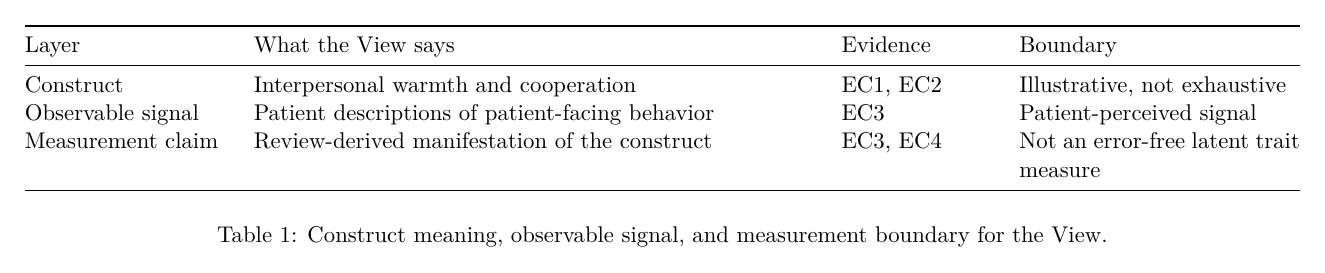
\includegraphics[width=0.94\linewidth]{assets/display-1.png}\end{center}
QBt1-Display2 is the two-panel illustration. Its current raster is embedded below; click QBt1-Display2 and the same preview appears first, before its panel bindings, files, and independent acceptance state.

\begin{center}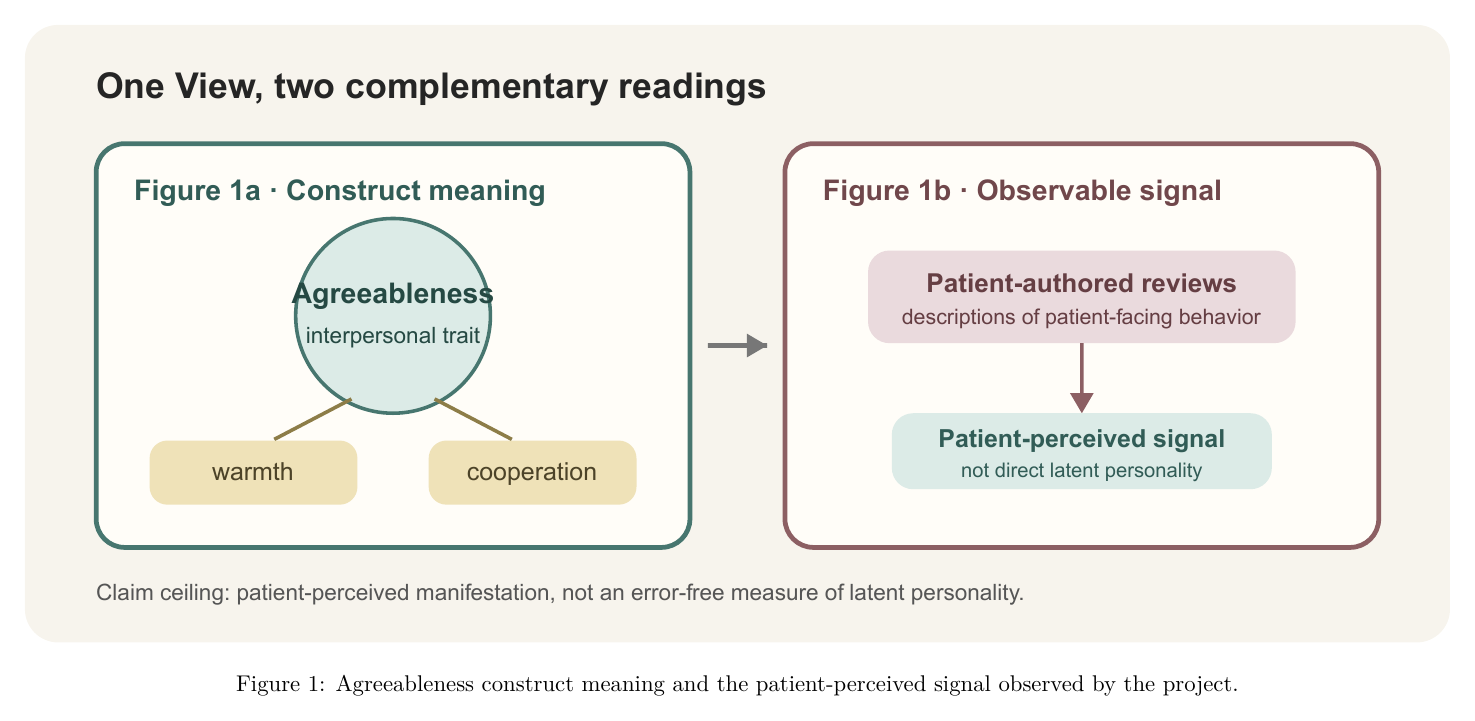
\includegraphics[width=0.94\linewidth]{assets/display-2.png}\end{center}
Each output also carries preview.pdf as the printable inspection surface. PNG is shown inline because it renders reliably in the Board browser; PDF remains linked in the Card at full fidelity.

Each authored output folder is also a complete generic renderer unit. output.md owns the View-level semantic judgment; intake/ binds approved evidence or context; recipe/ records reproducibility; candidates/, assets/, and versions/ separate alternatives, the winner, and history. No second Display adapter folder is created.

The two Displays remain separate because a person can inspect and accept them independently.

They remain inside one View because both are outputs selected from the same named View body.

QBt1-Display1 and QBt1-Display2 are the only required outputs in this specimen; prose packs and evidence ledgers are optional outputs, not universal folders.

\section*{4 · Consumers}
The outgoing side: consumers may link to the whole View or to selected Displays, and the View exposes that relationship before handoff.

\begin{Verbatim}[fontsize=\small]
View ─▶ whole-View consumer
  └──▶ QBt1-Display1/2 consumer + placement + gate state
\end{Verbatim}
The Main Results section plans to consume QBt1-Display1 for its construct-interpretation passage.

\begin{quote}\footnotesize\textbf{Evidence card.} Card Main Results section: C1 · Consumer · Target Page: S-Main-4 · Binding: QBt-page-types/consumer/S-Main-4-results.md. Uses: QBt1-Display1. Placement: Results / construct interpretation. Status: planned, blocked on View and Display acceptance.\end{quote}
Other legal consumers include Appendix sections, Narrative pages, reports, and applications.

A consumer may still reach a Probe directly when its own contract allows it; the View route is the normal human-readable handoff, not a ban on every direct link.

\section{References}\begin{itemize}
\item John, Oliver P.; Srivastava, Sanjay (1999). The Big-Five Trait Taxonomy: History, Measurement, and Theoretical Perspectives. Handbook of Personality: Theory and Research
\end{itemize}
\end{document}
